\documentclass[10pt]{beamer}

\usepackage[backend=bibtex,firstinits=true,style=verbose-inote,citestyle=authortitle]{biblatex}
\usepackage{bm}
\usepackage{graphicx}
\usepackage{mathtools}
\usepackage{subcaption}
\usepackage{makecell}
\usepackage{xcolor}
\newcommand{\expect}[2][]{
\ifthenelse{\equal{#1}{}}{
\mathbb{E}\left[#2\right]
}{
\underset{#1}{\mathbb{E}}\left[#2\right]
}}

\newcommand{\cov}[2][]{
\ifthenelse{\equal{#1}{}}{
\text{Cov}\left[#2\right]
}{
\underset{#1}{\text{Cov}}\left[#2\right]
}}


\newcommand{\var}[2][]{
\ifthenelse{\equal{#1}{}}{
\text{Var}[#2]
}{
\underset{#1}{\text{Var}}[#2]
}}

\newcommand{\loss}[2][]{
\ifthenelse{\equal{#1}{}}{
\mathcal{L}(#2)
}{
\mathcal{L}_{#1}(#2)
}}

\newcommand{\kl}[2]{
\text{D}_\text{KL}[#1 \parallel #2]
}

\newcommand{\R}{\mathbb{R}}
%\newcommand{\Prob}{\mathbb{P}}

\newcommand{\1}[1]{\mathds{1}\{#1\}}


%\usecolortheme{dolphin}
\setbeamertemplate{navigation symbols}{}
\setbeamertemplate{section in toc}{\inserttocsectionnumber.~\inserttocsection}
\addbibresource{xlnet.bib}

\title{XLNet: Generalized Autoregressive Pretraining for Language Understanding\footnote{\citepaper{xlnet}}\vspace{-3.0em}}
%\subtitle{(in images and text)}
%\author{Ivan Skorokhodov}
\date{June 21, 2019}
\logo{
\includegraphics[height=1cm]{images/ipavlov-logo.png}}

\newcommand{\citepaper}[1]{\citetitle{#1} by \citeauthor{#1}}

%\graphicspath{{./images}}

%\usetheme{lucid}
\begin{document}

\begin{frame}
    \titlepage
    \centering
    
\includegraphics[width=0.6\textwidth]{images/sad-bert.jpg}
\end{frame}


\section{Current methods}
\begin{frame}
\frametitle{What problems\footnote{besides obesity} BERT has?}

\begin{enumerate}
    \item\pause It predicts MASK tokens independently, i.e.
$p(\bm{\tilde{x}} | \bm{\hat x}) = \prod_{i=1}^T p(\tilde{x}_i | \bm{\hat x})$, where $\bm{\tilde x}, \bm{\hat x}$ are masked and unmasked subsequences of $\bm x$.  It's a big deal, because in reality:
    \[
    p(\text{New}, \text{York} | \bm{\hat x}) = p(\text{New} | \bm{\hat x}) \cdot p(\text{York} | \text{New}, \bm{\hat x}) \neq p(\text{New} | \bm{\hat x}) \cdot p(\text{York} | \bm{\hat x})
    \]
    \pause\item In test time we do not have MASK tokens, which is train-test discrepancy!\footnote{That's why we also predict non-mask tokens during pretraining.}
    \item\pause Using large contexts is very costly $O(n^2)$.
\end{enumerate}

\end{frame}


\begin{frame}
    \frametitle{What problems language models have?}
    
    \begin{itemize}
        \item\pause We can train them either forward or backward\footnote{or bidirectionally with simple concatenation, like ELMO}
        \item\pause $\Longrightarrow$ model is not trained to use the whole context
        \item\pause $\Longrightarrow$ it's bad, because such an information is very useful for some tasks
    \end{itemize}
\end{frame}

\begin{frame}
    \frametitle{XLNet to the rescue}
    \begin{itemize}
        \item\pause Let $\mathcal{Z}_T$ be a set of all possible permutations of a sequence of length $T$ (so it has $T!$ elements).
        \item\pause Note that we can decompose $p(\bm x)$ via chain rule in an arbitrary order:
        \begin{equation*}
        \begin{split}
        p(\bm x) &= p(x_1, x_2, x_3) \\
        &= p(x_1) p(x_2 | x_1) p(x_3 | x_1, x_2) \\
        &= p(x_2) p(x_3 | x_2) p(x_1 | x_2, x_3) \\
        &= ...
        \end{split}
        \end{equation*}
        
        \item\pause Which order is the best for our task? Forward? Backward?
        \item\pause All of them:
        \[
        \mathcal{L}_{\text{XLNet}}(\theta) = -\expect[\bm z \sim \mathcal{Z}_T]{\log p_\theta(\bm x)} = -\expect[\bm z \sim \mathcal{Z}_T]{\sum_{t=1}^T \log p_\theta(x_{z_t} | \bm x_{\bm z_{< t}})}
        \]
        %\footnote{Excuse me, sir, do you have a moment to talk about prior for $z$?}
        \item\pause Is this an upper bound for a true loss? Yes:
        \[
        \expect[\bm z]{\log p(\bm x | \bm z)} \leq \log \expect[\bm z]{p(\bm x | \bm z)} = \log p(\bm x)
        \]
    \end{itemize}
\end{frame}

\begin{frame}
    \frametitle{How does it look like in practice (1/3)?}

    \begin{itemize}
        \item\pause It's straight-forward how to decode the sequence in the required order $\bm z$: just use proper masks
    \end{itemize}
\pause
\begin{figure}
    \centering
    \begin{subfigure}[b]{0.49\textwidth}
        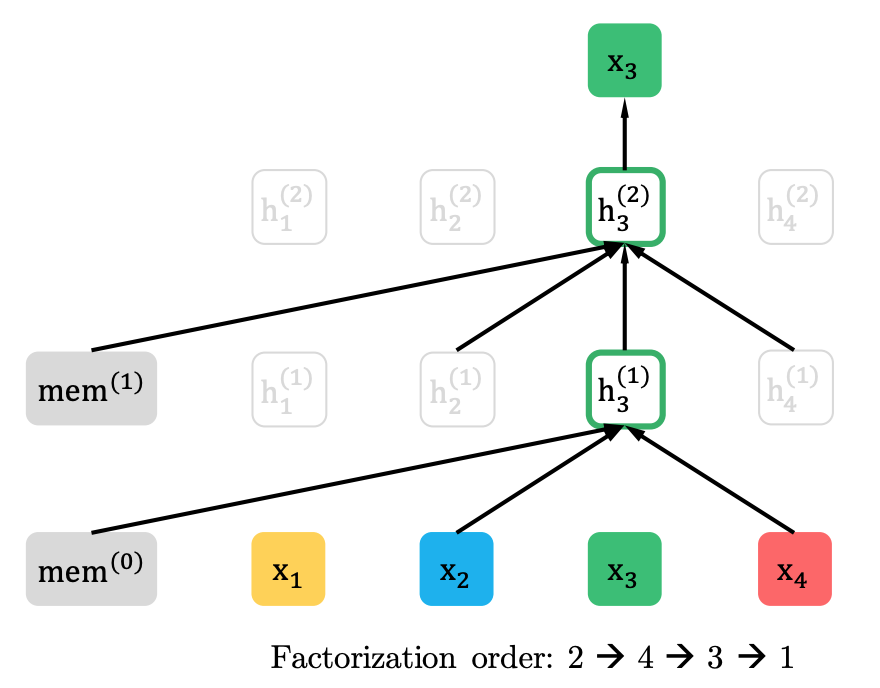
\includegraphics[width=\textwidth]{images/order-example-1.png}
        %\caption{Example of decoding $x_3$ in permutation order $z = 2 \to 4 \to 3 \to 1$}
    \end{subfigure}
    \begin{subfigure}[b]{0.49\textwidth}
        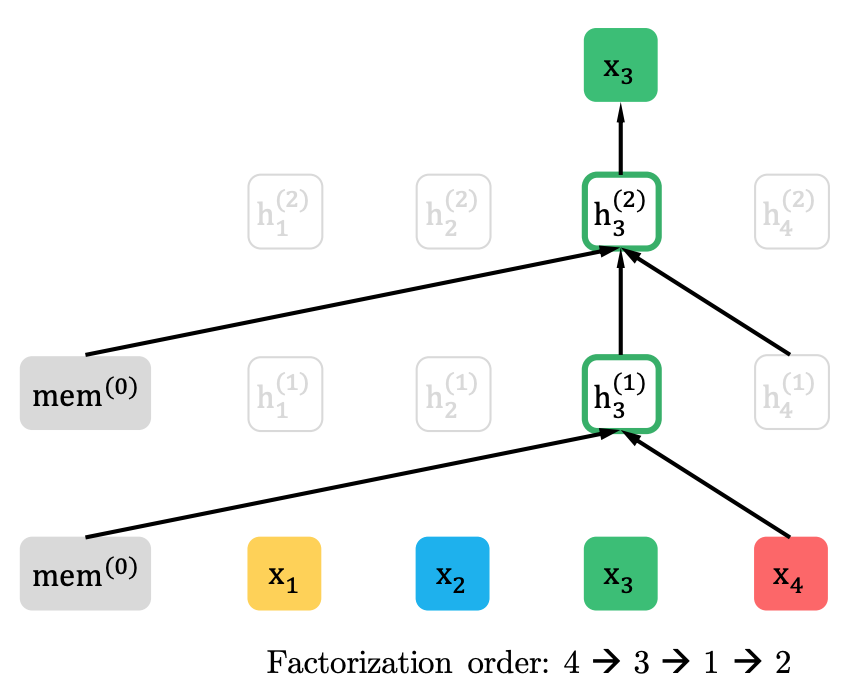
\includegraphics[width=\textwidth]{images/order-example-2.png}
        %\caption{Example of decoding $x_3$ in permutation order $z = 4 \to 3 \to 1 \to 2$}
    \end{subfigure}
    \caption{Example of prediction token $x_3$ for different permutation orders $\bm z$.}
\end{figure}
\end{frame}


\begin{frame}
\frametitle{How does it look like in practice (2/3)?}
\begin{itemize}
    \item\pause But we cannot predict ``next'' token like we do in language models!
    \item\pause Because we have many possible permutations, the same hidden state will be used to predict different tokens:
\[
\begin{rcases}
\bm z^{(1)} = (\textcolor{blue}{3, 4, 2}, \textcolor{red}{1,5}) \\
\bm z^{(2)} = (\textcolor{blue}{3, 4, 2}, \textcolor{red}{5,1})  
\end{rcases}
\Longrightarrow
\begin{cases}
p(x_1 = s | x_3, x_4, x_2) = \frac{\exp \left(e(x)^{\top} h_{\theta}\left(\mathbf{x}_{\mathbf{z}}<t\right)\right)}{\sum_{x^{\prime}} \exp \left(e\left(x^{\prime}\right)^{\top} h_{\theta}\left(\mathbf{x}_{\mathbf{z}<t}\right)\right)} \\
p(x_5 = s | x_3, x_4, x_2) = \frac{\exp \left(e(x)^{\top} h_{\theta}\left(\mathbf{x}_{\mathbf{z}}<t\right)\right)}{\sum_{x^{\prime}} \exp \left(e\left(x^{\prime}\right)^{\top} h_{\theta}\left(\mathbf{x}_{\mathbf{z}<t}\right)\right)}
\end{cases}
\]
    \item\pause Solution? \pause Predict token from additional [MASK] embedding.
\end{itemize}
\end{frame}

\begin{frame}
    \frametitle{How does it look like in practice (3/3)?}
    \begin{figure}
        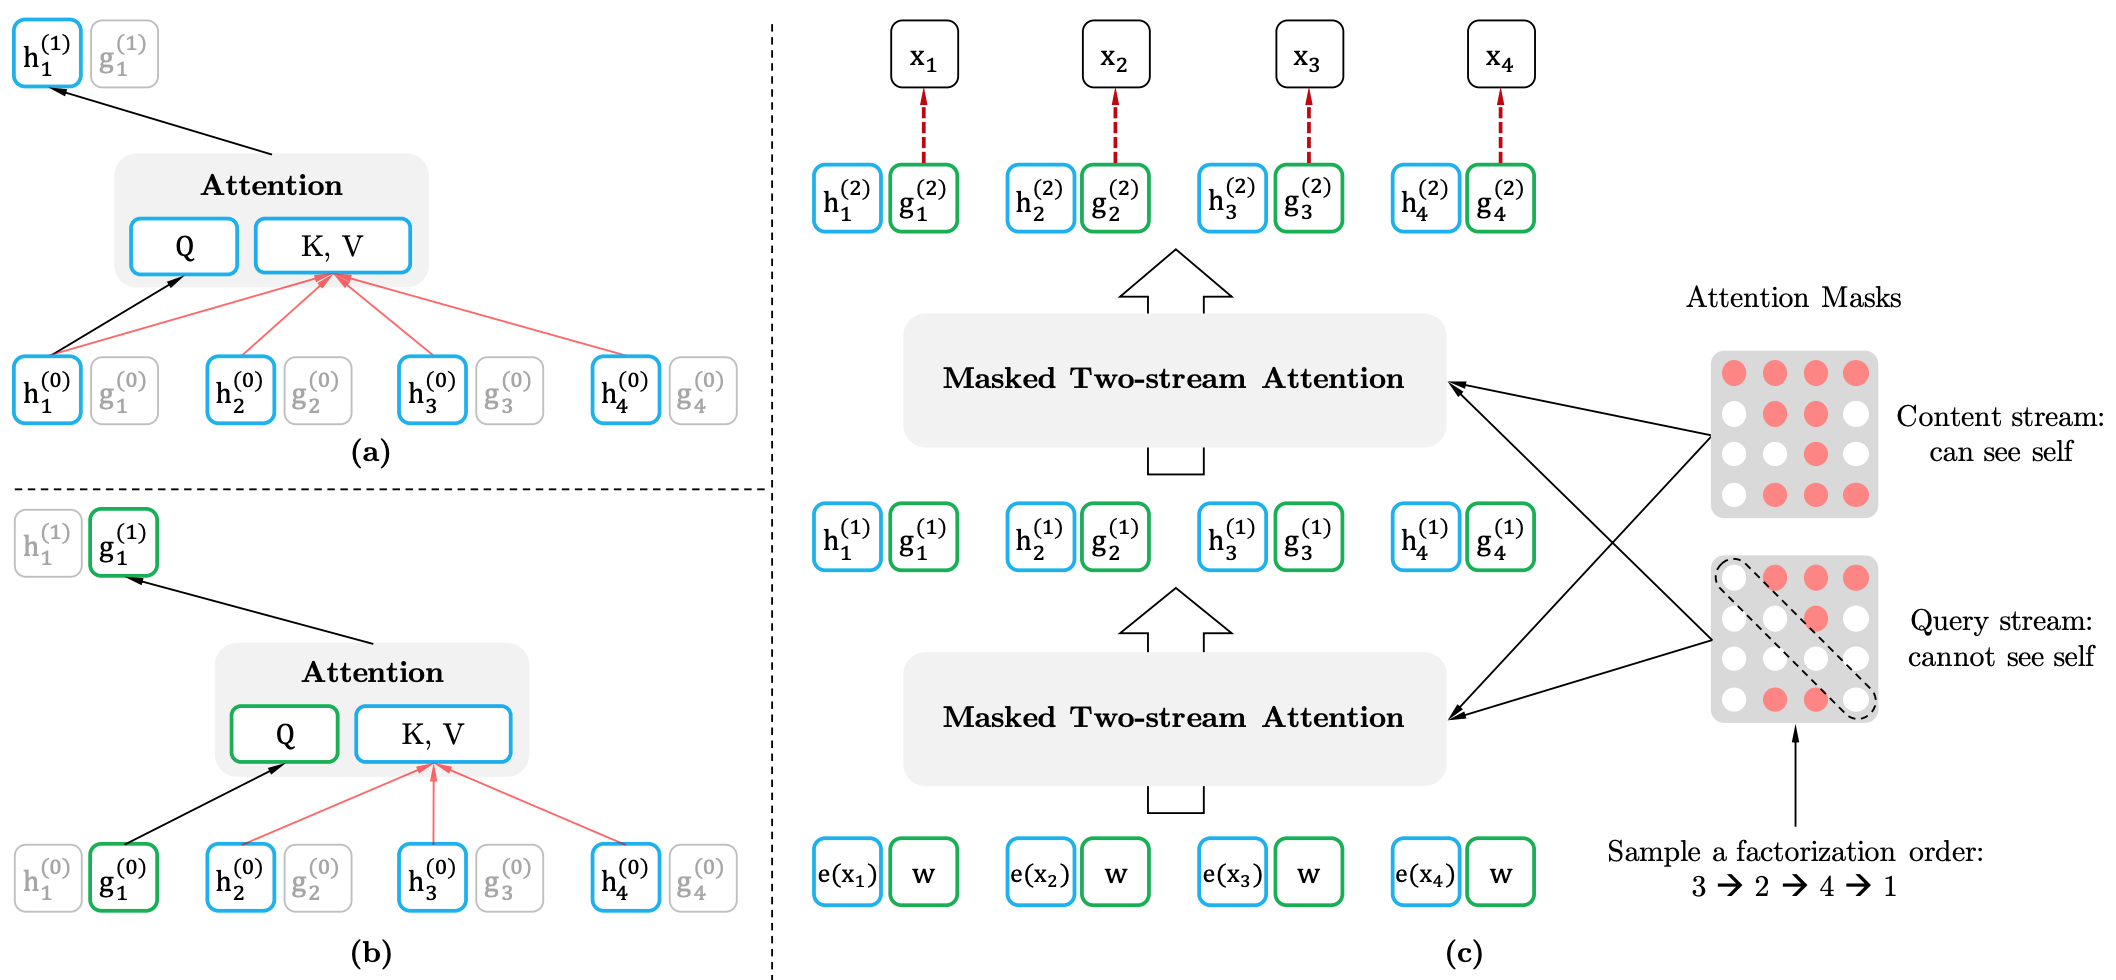
\includegraphics[width=\textwidth]{images/two-stream-self-attention.png}
        \caption{Two-stream self-attention (copy pasted for intensive hand waving).}
    \end{figure}
\end{frame}


\begin{frame}
    \frametitle{Training details}
    \begin{itemize}
        \item\pause For each sentence in a batch take a random permutation $\bm z \in \mathcal{Z}_T$ for decoding.
        \item\pause Initialize [MASK] tokens with trained embeddings.
        \item\pause Use forward/backward pass for each half of the batch (explained later).
        \item\pause Mask around 15\% of tokens (because otherwise it will be hard to train).
        \item\pause We use [A, SEP, B, SEP, CLS] like in BERT.
        \item\pause We use relative segment encoding: $a_{ij}^{\text{final}} = a_{ij} + (\bm q_i + \bm b)^\top \bm s_{ij}$, where $\bm q_i$ is our query, $\bm b$ is a learned head-specific vector, $\bm s_{ij} = \bm s_-$ or $\bm s_+$ if $i$ is in the same context as $j$ or not.
    \end{itemize}
\end{frame}

\begin{frame}
    \frametitle{Relative positional encoding}
    \framesubtitle{(from Transformer-XL)}
    \begin{itemize}
        \item\pause Key idea: make information about position be dependent only on relative positions between objects, regardless where they are placed in the sequence
        \item Why do we need this? \pause To attend on memory without much trouble (memory usually has the same positional embeddings).
        \item\pause Imagine we have hidden states $\bm e_i, \bm e_j$. We add positional embeddings to them: $\bm h_i = \bm e_i + \bm p_i$ and $\bm h_j = \bm e_j + \bm p_j$
    \end{itemize}
\pause Then normal attention of $\bm h_i$ on $\bm h_j$ is computed as
\begin{equation*}
\begin{split}
\text{Attn}(\bm h_i, \bm h_j)
&= \langle W_q \bm h_i, W_k \bm h_j \rangle = \langle W_q (\bm e_i + \bm p_i), W_k (\bm e_j + \bm p_j) \rangle \\
&= \bm e_i^\top W_q^\top W_k \bm e_j + \bm e_i^\top W_q^\top W_k \bm p_j + \bm p_i^\top W_q^\top W_k \bm e_j + \bm p_i^\top W_q^\top W_k \bm p_j
\end{split}
\end{equation*}

Relative positional encoding just changes attention mechanism to:
\begin{equation*}
\begin{split}
\text{Attn}^{\text{rel}}(\bm h_i, \bm h_j)
&= \bm e_i^\top W_q^\top W_k^{\textcolor{red}{e}} \bm e_j + \bm e_i^\top W_q^\top W_k^{\textcolor{red}{r}} \bm p_{\textcolor{red}{i-j}} + \textcolor{blue}{\bm u}^\top W_k^{\textcolor{red}{e}} \bm e_j + \textcolor{blue}{\bm v}^\top W_k^{\textcolor{red}{r}} \bm p_{\textcolor{red}{i-j}}
\end{split}
\end{equation*}

\end{frame}

\begin{frame}
    \frametitle{Adding memory (aka ``recurrence mechanism'')}
    \framesubtitle{(from Transformer-XL)}
    
    \begin{itemize}
        \item When we have really large sequence, we can process it segment by segment
        \item When previous segment is processed, put it into cache and attend as embeddings like we do in machine translation
    \end{itemize}
\end{frame}

\begin{frame}
    \frametitle{Quiz time!}
    \begin{itemize}
        \item\pause How many TPUs v3 were used? \pause --- 512
        \item\pause How long did the thing trained? \pause --- 2.5 days\footnote{And authors said that the model still underfit after 500K steps (but performance on downstream tasks didn't improve)}
        \item\pause What was the batch size? \pause --- 2048
        \item\pause What optimizer did they use? \pause --- Adam
    \end{itemize}
\end{frame}

\begin{frame}
    \frametitle{TODO}
I didn't have enough time to copy-paste tables from scores and ablation study, so let's open the paper and see them manually.
\end{frame}

\begin{frame}
    \frametitle{Things I didn't get}
    \begin{itemize}
        \item Span-based prediction?
    \end{itemize}
\end{frame}

\end{document}
